\documentclass[12pt]{article}
\usepackage[hidelinks]{hyperref}    
\usepackage[all]{hypcap}
\usepackage{amssymb}
\usepackage{amsmath}
\usepackage{graphicx}
\graphicspath{{../images/}}
\title{\textbf{Analisi Matematica\\Limiti}}
\date{07 Ottobre 2024}
\author{Andrea Malvezzi}
\begin{document}
\maketitle
\pagebreak
\tableofcontents
\pagebreak
\section{La nozione di limite}
\subsection{Introduzione}
Avendo:
\[
    x_0 \in \mathbb{R}, r \in \mathbb{R} : r > 0 \text{ (molto piccolo)}
\]
Si dice intorno di $x_0$ la parte di piano sferica avente centro $x_0$ e raggio $r$, tale che:
\begin{equation}
    I_r(x_0) = x \in \mathbb{R} : | x - x_0 | < r \label{def:intorno}
\end{equation}
Inoltre un punto in un insieme $A$ è detto di accumulazione quando facendo l'intersezione tra $A$ stesso e l'intorno del punto MENO il punto stesso, si ottiene un insieme non-vuoto. Ovvero:
\begin{equation}
    A \cap (I_r(\overline{x}) - {\overline{x}}) != \emptyset \label{def:punto_accumulazione}
\end{equation}
E l'insieme di tutti i punti di accumulazione di un insieme $A$, anche detto \textbf{Derivato di $A$}, si indica con la seguente:
\begin{equation}
    \mathbb{A} = {\overline{x} \in \mathbb{R} : \dots \text{ (definizione di punto di accumulazione, vedi (\ref{def:punto_accumulazione}))}} 
\end{equation}
\pagebreak
\subsubsection{Esempi di punto di accumulazione}
A seguire alcuni esempi di punti di accumulazione di una funzione definita tra $1$ (escluso) e $6$ (incluso).
\begin{figure}[!htb]
    \centering
    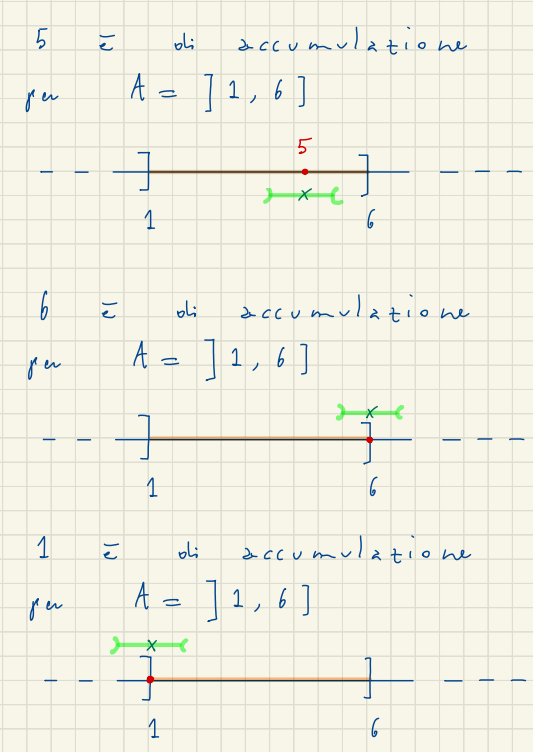
\includegraphics[width=1\textwidth, height=.7\textheight,keepaspectratio]{lezione_7/esempi_punti_accumulazione.png}
    \begin{center}
        \caption{\label{fig:esempi_punti_accumulazione}Esempi di punti di accumulazione di una funzione.}
    \end{center}
\end{figure}
\pagebreak
\subsection{Ma perché si toglie il centro?}
Il centro di un intorno si rimuove per esplicitare dal punto di vista matematico l'atto di avvicinarsi indefinitamente a tale punto, all'interno della funzione. Se non si rimuovesse tale valore, nell'esempio presentato a seguito $7$ sarebbe punto di accumulazione altrimenti.
\begin{figure}[!htb]
    \centering
    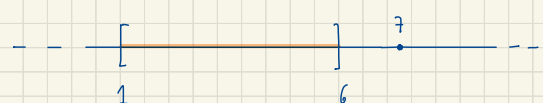
\includegraphics[width=1\textwidth, height=.7\textheight,keepaspectratio]{lezione_7/rimozione_centro_intorno.png}
    \begin{center}
        \caption{\label{fig:rimozione_centro}Esempio di punto non di accumulazione ($7$).}
    \end{center}
\end{figure}
\subsection{Definizione di limite finito al finito}
Avendo:
\[
    f: A \rightarrow \mathbb{R}, \text{ } x_0 \in \mathbb{D}(A), \text{ } l \in \mathbb{R}
\]
Si dice che:
\[
    \lim_{x \to x_0} f(x) = l
\]
se:
\begin{equation}
    \forall \theta > 0, \exists \delta = \delta(x_0, \theta)>0 : \forall x \in a: 0 <  0 < |x - x_0| < \delta
\end{equation}
\section{Teoremi utili per operare con i limiti}
\subsection{Teorema di permanenza del segno}
Avendo:
\[
    f: A \rightarrow \mathbb{R}, \text{ } \overline{x} \in \mathbb{D}(A), \text{ } \lim_{x \to \overline{x}} f(x) = l \in \mathbb{R}, \text{ } l > 0 \text{ oppure } l < 0 \text{ (due casi)}
\]
Allora:
\begin{equation}
    \exists \delta > 0: \forall x \in A, \text{ } \overline{x} - \delta < x < \overline{x} + \delta, \text{ } x != \overline{x}   \label{teo:permanenza_segno}
\end{equation}
Che essenzialmente significa che se si ha un limite tendente ad $\overline{x}$, vicino a $\overline{x}$ la funzione studiata avrà un segno costante.
\subsection{Teorema del confronto (due carabinieri)}
Avendo:
\[
    f, g, h : A \rightarrow \mathbb{R}, \text{ } x_0 \in \mathbb{D}(A)
\]
Supponiamo che:
\begin{equation}
    \lim_{x \to x_0} g(x) = \lim_{x \to x_0} h(x) = l \in \mathbb{R} \label{teo:carabinieri_suppose}
\end{equation}
Allora:
\begin{equation}
    \exists \delta > 0: g(x) \leq f(x) \leq h(x), \text{ } \forall x \in [A \cup I_\delta(x_0)] - \{x_0\} \label{teo:carabinieri_then}
\end{equation}
Ed infine:
\begin{equation}
    \lim_{x \to x_0} f(x) = l \label{teo:carabinieri_end}
\end{equation}
\subsection{Altre proprietà}
Valgono inoltre le seguenti proprietà, utili a scomporre i limiti:
\begin{figure}[!htb]
    \centering
    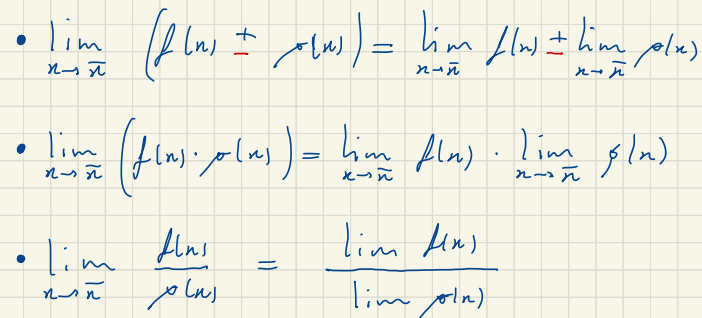
\includegraphics[width=1\textwidth, height=.7\textheight,keepaspectratio]{lezione_7/prop_limiti.png}
    \begin{center}
        \caption{\label{fig:proprietà_limiti}Proprietà dei limiti.}
    \end{center}
\end{figure}
\section{Il limite più importante della goniometria}
Il limite più importante della goniometria è:
\begin{equation}
    \lim_{x \to 0} \dfrac{\sin{x}}{x} = 1 \label{lim:seno}
\end{equation}
E per dimostrare tale limite occorre anzitutto assumere che:
\[
    0 < x < \dfrac{\pi}{2}
\]
E poi passare alla rappresentazione geometrica:
\begin{figure}[!htb]
    \centering
    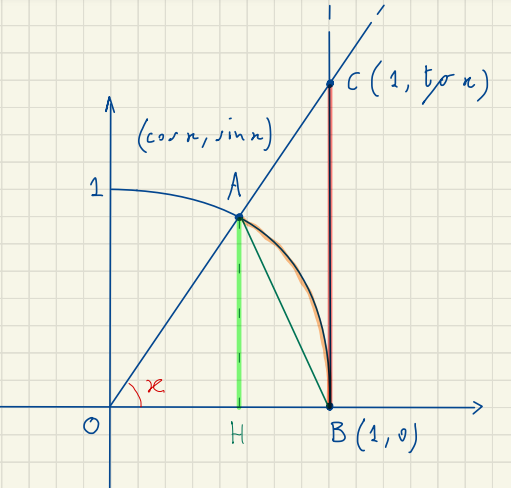
\includegraphics[width=1\textwidth, height=.5\textheight,keepaspectratio]{lezione_7/limite_seno_geometria.png}
    \begin{center}
        \caption{\label{fig:lim_seno_geometria}Si intuisce che \(\overset{\triangle}{AOH}\). e \(\overset{\triangle}{BOC}\) siano simili.}
    \end{center}
\end{figure}
\pagebreak
\\Ora, intuitivamente, si dimostra che:
\[  
    % TODO:sistema il cappello
    \overline{AH} \leq |\overset{\cup}{AB}| \leq \overline{BC}
\]
Ovvero, passando agli equivalenti nella goniometria:
\[
    \sin{x} \leq x \leq \tan{x}
\]
Dividiamo ora per $\sin{x}$ per ottenere:
\[
    \dfrac{\sin{x}}{sin{x}} \leq \dfrac{n}{sin{x}} \leq \dfrac{\tan{x}}{\sin{x}} = \dfrac{sin{x}}{cos{x}} \cdot \dfrac{1}{\sin{x}} = \dfrac{1}{\cos{x}}
    % TODO:slide 39
\]
\end{document}